\section{Simulation Analysis}
\label{sec:simulation}

\subsection{Operating Point Analysis}

Once again, the simulated operating points were computed to check if the transistors were working in the correct regions. \par
Table  shows the simulated operating point results for the circuit
under analysis.

\begin{table}[h]
  \centering
  \begin{tabular}{|l|r|}
    \hline    
    {\bf Name} & {\bf Value [V]} \\ \hline
    vce & 7.969251e+00\\ \hline
vbe & 6.986238e-01\\ \hline
vo1 & 8.654746e+00\\ \hline
vec & 9.397377e+00\\ \hline
veb & 7.426318e-01\\ \hline
vo2 & 9.397377e+00\\ \hline

  \end{tabular}
  \caption{Operating point}
  \label{tab:OP_sim}
\end{table}
\FloatBarrier

Here the transistors are working in the Forward Active Region. The values are compared with the theoretical predictions in Section \ref{sec:sbs}.


\subsection{Frequency Analysis}
The frequency analysis was done in order to obtain the gain of the circuit as a function of the frequency. \par
The following plot shows the function we obtained for $V_{out}$.

\begin{figure}[h] \centering
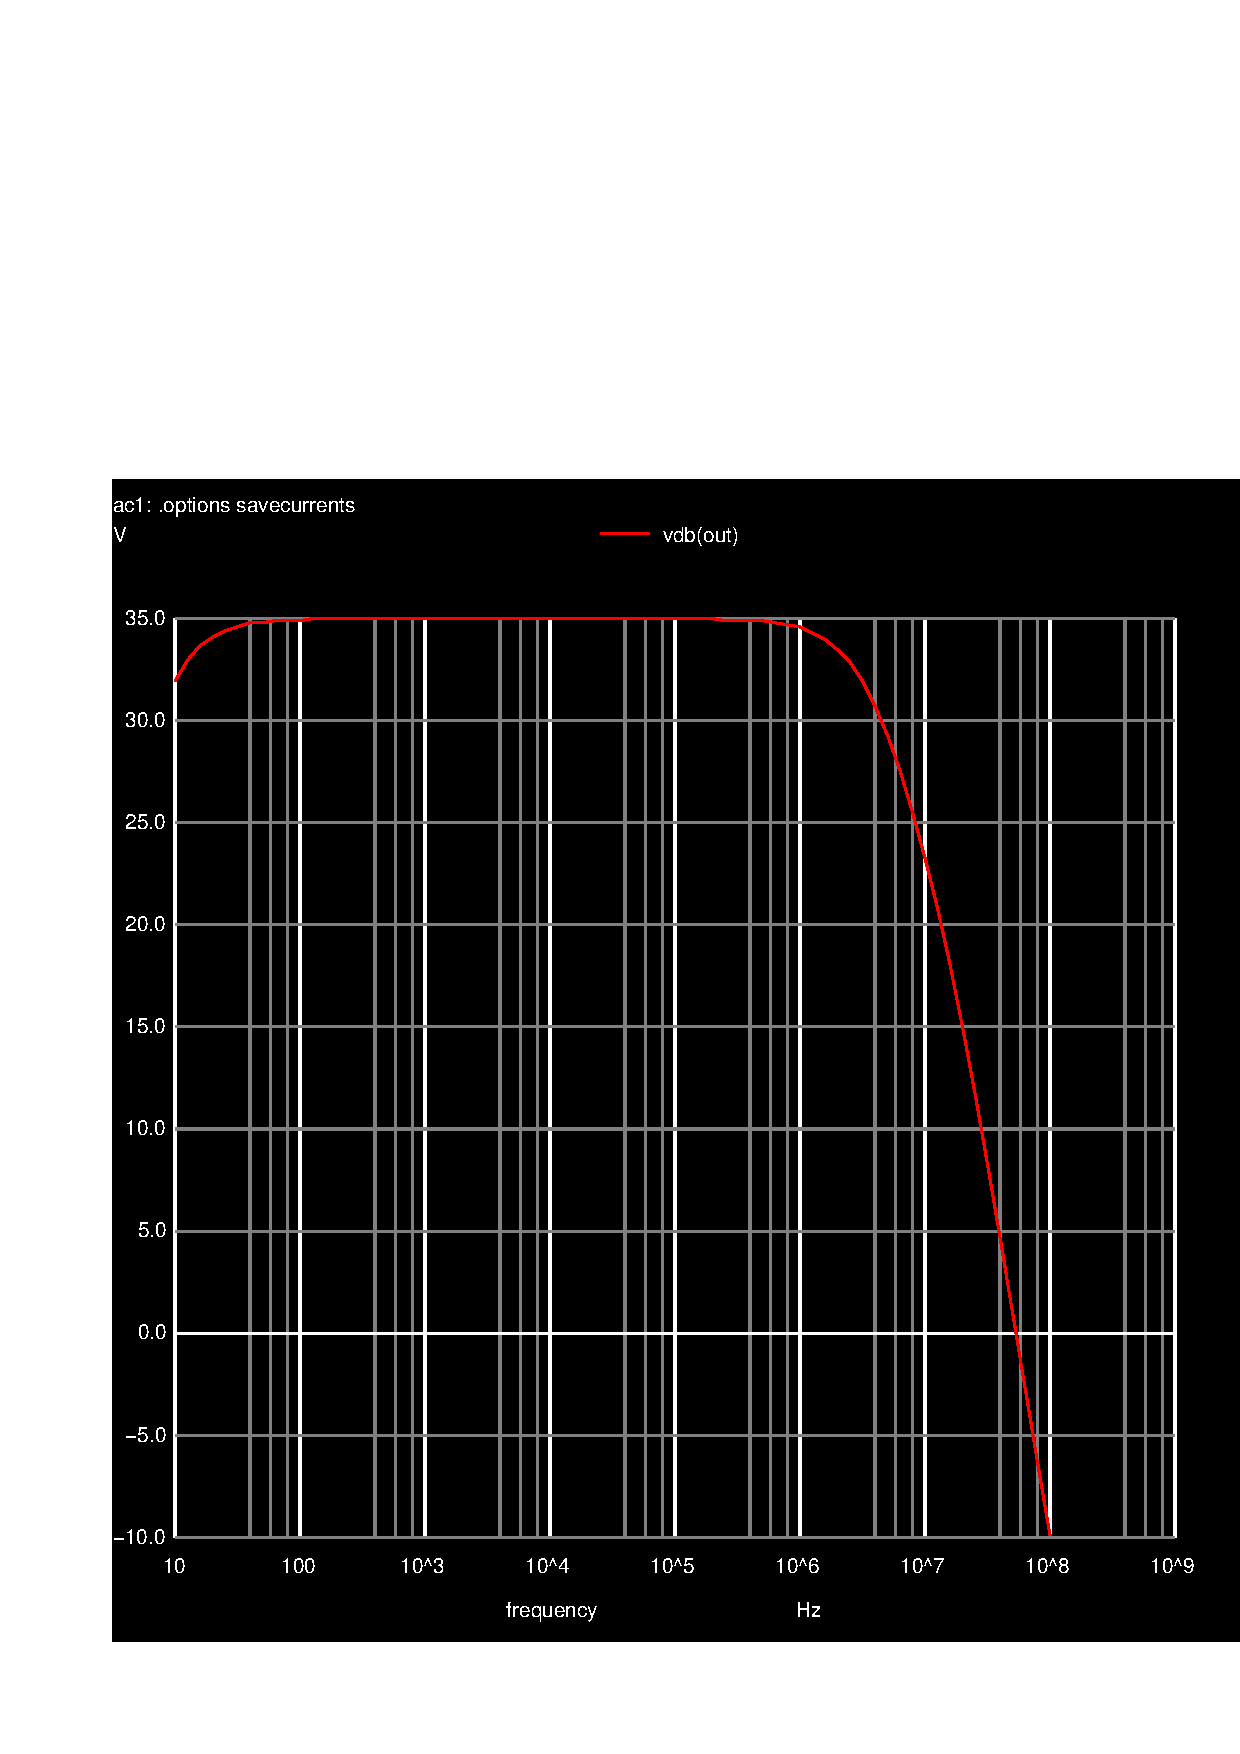
\includegraphics[width=0.5\linewidth]{vo2f.pdf}
\caption{vOUT (dB)}
\label{fig:vOUT}
\end{figure}
\FloatBarrier

From this analysis, we can also obtain the values for the upper and lower cut off frequencies, which allows us to compute the bandwidth. the input impedance and the output impedance, where we used a different circuit with $V_{IN}$ and $R_{IN}$ disconnected and an output voltage source. \par
The values obtained for the impedances and for the gain are presented in the following table. They are compared with the theoretical calculations in Section \ref{sec:sbs}.

\begin{table}[h]
  \centering
  \begin{tabular}{|l|r|}
    \hline    
    {\bf Name} & {\bf Value [$\Omega]$} \\ \hline
    z_in1 & 5.638527e+02,-8.44302e+01\\ \hline
gain & -7.85216e+01,-1.54185e+00\\ \hline
lco & 8.880418e+03\\ \hline
uco & 1.603742e+06\\ \hline
bandwith & 1.594862e+06\\ \hline
cost & 1.013002e+05\\ \hline
merit & -1.39209e-01,-2.73352e-03\\ \hline

  \end{tabular}
  \caption{Gain, input impedance and output impedance}
  \label{tab:IN_out_sim}
\end{table}
\FloatBarrier
Here we present the values of the cutt off frequencies and the value of the bandwidth. Once again, these are compared with the theoretical results in Section \ref{sec:sbs}.


\begin{table}[h]
  \centering
  \begin{tabular}{|l|r|}
    \hline    
    {\bf Name} & {\bf Value [Hz]} \\ \hline
    uco & 3.106930e+06\\ \hline
lco & 7.923603e+00\\ \hline
bandwith & 3.106922e+06\\ \hline

  \end{tabular}
  \caption{Bandwidth}
  \label{tab:Bandwith_sim}
\end{table}
\FloatBarrier

\subsection{Merit Figure}
In this section, we present the costs of the components and the total cost of the circuit, as well as the merit figure.

\begin{table}[h]
  \centering
  \begin{tabular}{|l|r|}
    \hline    
    {\bf Name} & {\bf Value [Mu]} \\ \hline
    cost & 8.116008e+03\\ \hline
merit & 2.707518e+03\\ \hline

  \end{tabular}
  \caption{Merit figure}
  \label{tab:OP}
\end{table}
\FloatBarrier

